% ---------------------------------------------------------------------
% -------------- PREAMBLE ---------------------------------------------
% ---------------------------------------------------------------------
\documentclass[12pt,a4paper,finnish,oneside]{article}
%\documentclass[12pt,a4paper,finnish,twoside]{article}
%\documentclass[12pt,a4paper,finnish,oneside,draft]{article} % luonnos, nopeampi

% Valitse 'input encoding':
%\usepackage[latin1]{inputenc} % merkistökoodaus, jos ISO-LATIN-1:tä.
\usepackage[utf8]{inputenc}   % merkistökoodaus, jos käytetään UTF8:a
% Valitse 'output/font encoding':
%\usepackage[T1]{fontenc}      % korjaa ääkkösten tavutusta, bittikarttana
\usepackage{ae,aecompl}       % ed. lis. vektorigrafiikkana bittikartan sijasta
% Kieli- ja tavutuspaketit:
\usepackage[english,swedish,finnish]{babel}
% Kurssin omat asetukset aaltosci_t.sty:
%\usepackage{aaltosci_t}
% Jos kirjoitat muulla kuin suomen kielellä valitse:
%\usepackage[finnish]{aaltosci_t}           
%\usepackage[swedish]{aaltosci_t}           
\usepackage[english]{aaltosci_t}           
% Muita paketteja:
\usepackage{alltt}
\usepackage{amsmath}   % matematiikkaa
\usepackage{calc}      % käytetään laskurien (counter) yhteydessä (tiedot.tex)
\usepackage{eurosym}   % eurosymboli: \euro{}
\usepackage{url}       % \url{...}
\usepackage{listings}  % koodilistausten lisääminen
\usepackage{algorithm} % algoritmien lisääminen kelluvina
\usepackage{algorithmic} % algoritmilistaus
\usepackage{hyphenat}  % tavutuksen viilaamiseen liittyvä (hyphenpenalty,...)
\usepackage{supertabular,array}  % useampisivuinen taulukko

% Koko dokumentin kattavia asetuksia:

% Tavutettavia sanoja:
%\hyphenation{vää-rin me-ne-vi-en eri-kois-ten sa-no-jen tavu-raja-ehdo-tuk-set}
% Huomaa, että ylläoleva etsii tarkalleen kyseisiä merkkijonoja, eikä
% ymmärrä taivutuksia. Paikallisesti tekstin seassa voi myös ta\-vut\-taa.

% Rangaistaan tavutusta (ei toimi?! Onko hyphenat-paketti asennettu?)
\hyphenpenalty=10000   % rangaistaan tavutuksesta, 10000=ääretön
\tolerance=1000        % siedetään välejä riveillä
% titlesec-paketti auttaa, jos tämän mukana menee sekaisin

% Tekstiviitteiden ulkoasu.
% Pakettiin natbib.sty/aaltosci.bst liittyen katso esim. 
% http://merkel.zoneo.net/Latex/natbib.php
% jossa selitykset citep, citet, bibpunct, jne.
% Valitse alla olevista tai muokkaa:
\bibpunct{(}{)}{;}{a}{,}{,}    % a = tekijä-vuosi (author-year)
%\bibpunct{[}{]}{;}{n}{,}{,}    % n = numero [1],[2] (numerical style)

% Rivivälin muuttaminen:
\linespread{1.24}\selectfont               % riviväli 1.5
%\linespread{1.24}\selectfont               % riviväli 1, kun kommentoit pois

% ---------------------------------------------------------------------
% -------------- DOCUMENT ---------------------------------------------
% ---------------------------------------------------------------------

\begin{document}

% -------------- Tähän dokumenttiin liittyviä valintoja  --------------

%\raggedright         % Tasattu vain vasemmalta, ei tavutusta
% ----------------- joitakin makroja ----------------------------------
%
% \newcommand{\sinunKomentosi}[argumenttienMäärä]{komennot%
% voiJakaaRiveille%
% jaArgumenttienViittaus#1,#2,#argumenttienMäärä}

% Joskus voi olla tarpeen kommentoida jotakin. Ei suositella. 
% Äläkä unohda lopulliseen! 
\newcommand{\Kommentti}[1]{\fbox{\textbf{OMA KOMMENTTI:} #1}}
% Käyttö: Kilometri on 1024 metriä. \Kommentti{varmista tämä vielä}.
% Eli newcommand:n komentosanan jälkeen hakasaluissa argumenttien lkm,
%  ja argumentteihin viitataa #1, #2, ...

%  Comment out this \DRAFT macro if this version no longer is one!  XXX
%\newcommand{\DRAFT}{\begin{center} {\it DRAFT! \hfill --- \hfill DRAFT!
%\hfill --- \hfill DRAFT! \hfill --- \hfill DRAFT!}\end{center}}

%  Use this \DRAFT macro in the final version - or comment out the 
%  draft-command
% \newcommand{\DRAFT}{~}

% %%%%%%%% MATEMATIIKKA %%%%%%%%%%%%%%%%%

% Määrätty integraali
\newcommand{\myInt}[4]{%
\int_{#1}^{#2} #3 \, \textrm{d}{#4}}

% http://kapsi.fi/jks/satfaq/
%\newcommand{\vii}{\mathop{\Big/}}
%\newcommand{\viiva}[2]{\vii\limits_{\!\!\!\!{#1}}^{\>\,{#2}}}
%%\[ \intop_0^{10} \frac{x}{x^2+1} \,\mathrm{d}x
%%= \viiva{0}{10} \frac{1}{2}\ln(x^2+1) \]

% matht.sty, Simo K. Kivelä, 01.01.2002, 07.04.2004, 19.11.2004, 21.02.2005
% Kokoelma matemaattisten lausekkeiden kirjoittamista helpottavia
% määrittelyjä.

% 07.04.2004 Muutama lisäys ja muutos tehty: \ii, \ee, \dd, \der,
% \norm, \abs, \tr.
%
% 19.11.2004 Korjattu määrittelyjä: \re, \im, \norm;
% lisätty \trp (transponointi), \hrm (hermitointi), \itgr (rakenteellinen
% integraali), ympäristö Cmatrix (hakasulkumatriisi);
% vanha transponointi \tr on mukana edelleen, mutta ei suositella.

% Pakotettu rivinvaihto, joka voidaan tarvittaessa määritellä
% uudelleen: 

%\newcommand{\nl}{\newline}

% Logiikan symboleja (<=> ja =>) hieman muunnettuina:

%\newcommand{\ifftmp}{\;\Leftrightarrow\;}
%\newcommand{\impltmp}{\DOTSB\;\Rightarrow\;}

% 'siten, että' -lyhenne ja hattupääyhtäläisyysmerkki vastaavuuden
% osoittamiseen: 

%\newcommand{\se}{\quad \text{siten, että} \quad}
%\newcommand{\vs}{\ {\widehat =}\ }

% Lukujoukkosymbolit:

%\newcommand{\N}{\ensuremath{\mathbb N}}
%\newcommand{\Z}{\ensuremath{\mathbb Z}}
%\newcommand{\Q}{\ensuremath{\mathbb Q}}
%\newcommand{\R}{\ensuremath{\mathbb R}}
%\newcommand{\C}{\ensuremath{\mathbb C}}

% Reaali- ja imaginaariosa, imaginaariyksikkö:

%\newcommand{\re}{\operatorname{Re}}
%\newcommand{\im}{\operatorname{Im}}
%\newcommand{\ii}{\mathrm{i}}

% Differentiaalin d, Neperin luku:

%\newcommand{\dd}{\mathrm{d}}
%\newcommand{\ee}{\mathrm{e}}

% Vektorimerkintä, joka voidaan tarvittaessa määritellä uudelleen
% (tämä tekee vektorit lihavoituina):

%\newcommand{\V}[1]{{\mathbf #1}}

% Kulmasymboli:

%\renewcommand{\angle}{\sphericalangle}

% Vektorimerkintä, jossa päälle pannaan iso nuoli;
% esimerkiksi \overrightarrow{AB} (tämmöisiä olemassaolevien
% symbolien uudelleenmäärittelyjä ei kyllä pitäisi tehdä):

%\renewcommand{\vec}[1]{\overrightarrow{#1}}

% Vektoreiden vastakkaissuuntaisuus:

%\newcommand{\updownarrows}{\uparrow\negthinspace\downarrow}

% Itseisarvot ja normi:

%\newcommand{\abs}[1]{{\left\vert#1\right\vert}}
%\newcommand{\norm}[1]{{\left\Vert #1 \right\Vert}}

% Transponointi ja hermitointi:

%\newcommand{\trp}[1]{{#1}\sp{\operatorname{T}}}
%\newcommand{\hrm}[1]{{#1}\sp{\operatorname{H}}}

% Vanha transponointi; jäljellä yhteensopivuussyistä, ei syytä käyttää.
%\newcommand{\tr}{{}^{\text T}}

% Arcus- ja area-funktiot, jossa päähaara osoitetaan nimen päälle
% vedetyllä vaakasuoralla viivalla (alkaa olla vanhentunutta,
% voitaisiin luopua):

%\newcommand{\arccot}{\operatorname{arccot}}
%\newcommand{\asin}{\operatorname{\overline{arc}sin}}
%\newcommand{\acos}{\operatorname{\overline{arc}cos}}
%\newcommand{\atan}{\operatorname{\overline{arc}tan}}
%\newcommand{\acot}{\operatorname{\overline{arc}cot}}

%\newcommand{\arsinh}{\operatorname{arsinh}}
%\newcommand{\arcosh}{\operatorname{arcosh}}
%\newcommand{\artanh}{\operatorname{artanh}}
%\newcommand{\arcoth}{\operatorname{arcoth}}
%\newcommand{\acosh}{\operatorname{\overline{ar}cosh}}

% Signum, syt, pyj:

%\newcommand{\sg}{\operatorname{sgn}}
%\renewcommand{\gcd}{\operatorname{syt}}
%\newcommand{\lcm}{\operatorname{pyj}}

% Lyhennemerkintöjä: derivaatta, osittaisderivaatta, gradientti,
% derivaattaoperaattori, vektorin komponentti, integraalin ylä- ja
% alasumma, Suomessa (ja Saksassa?) käytetty integraalin sijoitus-
% merkintä, integraali (rakenteellinen määrittely):

%\newcommand{\der}[2]{\frac{\dd #1}{\dd #2}}
%\newcommand{\osder}[2]{\frac{\partial #1}{\partial #2}}
%\newcommand{\grad}{\operatorname{grad}}
%\newcommand{\Df}{\operatorname{D}} 
%\newcommand{\comp}{\operatorname{comp}}
%\newcommand{\ys}[1]{\overline S_{#1}}
%\newcommand{\as}[1]{\underline S_{#1}}
%\newcommand{\sijoitus}[2]{\biggl/_{\null\hskip-6pt #1}^{\null\hskip2pt #2}} 
%\newcommand{\itgr}[4]{\int_{#1}^{#2}#3\,\dd #4}

% Matriiseja, joille voidaan antaa alkioiden sijoittamista sarakkeen
% vasempaan tai oikeaan reunaan tai keskelle osoittava lisäparametri
% (l, r tai c); ympärillä kaarisulut, hakasulut, pystyviivat (determinantti)
% tai ei mitään;
% esimerkiksi \begin{cmatrix}{ll}1 & -1 \\ -1 & 1 \end{cmatrix}:

%\newenvironment{cmatrix}[1]{\left(\begin{array}{#1}}{\end{array}\right)}
%\newenvironment{Cmatrix}[1]{\left[\begin{array}{#1}}{\end{array}\right]}
%\newenvironment{dmatrix}[1]{\left|\begin{array}{#1}}{\end{array}\right|}
%\newenvironment{ematrix}[1]{\begin{array}{#1}}{\end{array}}

% Kaunokirjoitussymboli:

%\newcommand{\Cal}{\mathcal}

% Isokokoinen summa:

%\newcommand{\dsum}[2]{{\displaystyle \sum_{#1}^{#2}}}

% Tuplaintegraali umpinaisen pinnan yli; korvataan jos parempi löytyy:
%\newcommand\oiint{\begingroup
% \displaystyle \unitlength 1pt
% \int\mkern-7.2mu
% \begin{picture}(0,3)
%   \put(0,3){\oval(10,8)}
% \end{picture}
% \mkern-7mu\int\endgroup}
       % Haetaan joitakin makroja

% Kieli:
% Kielesi, jolla kandidaatintyön kirjoitat: finnish, swedish, english.
% Tästä tulee mm. tietyt otsikkonimet ja kuva- ja taulukkoteksteihin 
% (Kuva, Figur, Figure), (Taulukko, Tabell, Table) sekä oikea tavutus.
%\selectlanguage{finnish}
%\selectlanguage{swedish}
\selectlanguage{english}

% Sivunumeroinnin kanssa pieniä ristiriitaisuuksia.
% Toimitaan pääosin lähteen "Kirjoitusopas" luvun 5.2.2 mukaisesti.
% Sivut numeroidaan juoksevasti arabialaisin siten että 
% ensimmäiseltä nimiölehdeltä puuttuu numerointi.
\pagestyle{plain}
\pagenumbering{arabic}
% Muita tapoja: kandiohjeet: ei numerointia lainkaan ennen tekstiosaa
%\pagestyle{empty}
% Muita tapoja: kandiohjeet: roomalainen numerointi alussa ennen tekstiosaa
%\pagestyle{plain}
%\pagenumbering{roman}        % i,ii,iii, samalla alustaa laskurin ykköseksi

% ---------------------------------------------------------------------
% -------------- Luettelosivut alkavat --------------------------------
% ---------------------------------------------------------------------

% -------------- Nimiölehti ja sen tiedot -----------------------------
%
% Nimiölehti ja tiivistelmä kirjoitetaan seminaarin mukaan joko
% suomeksi tai ruotsiksi (ellei erityisesti kielenä ole englanti). 
% Tiivistelmän voi suomen/ruotsin lisäksi kirjoittaa halutessaan
% myös englanniksi. Eli tiivistelmiä tulee yksi tai kaksi kpl.
%
% "\MUUTTUJA"-kohdat luetaan aaltosci_t.sty:ä varten.

\author{Tommi Jäske}

% Otsikko nimiölehdelle. Yleensä sama kuin seuraavana oleva \TITLE, 
% mutta jos nimiölehdellä tarvetta "kaksiosaiselle" kaksiriviselle
%\title{\LaTeX{}-pohja kandidaatintyötä varten ohjeiden kera ja varuilta 
%kokeillaan vähän ylipitkää otsikkoa}
% 2-osainen otsikko:
\title{Security in Microservice Architecture \\[5mm] - Impact of a Switch from Monolith to Microservices}

% Otsikko tiivistelmään. Jos lisäksi engl. tiivistelmä, niin viimeisin:
\TITLE{Turvallisuus mikropalveluarkkitehtuurissa\\[5mm] - Monoliitisesta arkkitehtuurista siirtyminen mikropalveluarkkitehtuuriin ja sen vaikutukset.}
%\TITLE{\LaTeX{} för kandidatseminariet med jättelång rubrik som fortsätter och
% fortsätter ännu}
\ENTITLE{Security in Microservice Architecture \\[5mm] - Impact of a Switch from Monolith to Microservices}
% 2-osainen otsikko korvataan täällä esim. pisteellä:
%\TITLE{\LaTeX{}-pohja kandidaatintyölle. Pitkiä rivejä kokeilun vuoksi.}

% Ohjaajan laitos suomi/ruotsi ja tarvittaessa eng (tiivistelmän kieli/kielet)
%\DEPT{Poimi tähän ohjaajasi laitos, DEPT, main.tex}
% suomi:
\DEPT{Tietotekniikan laitos}               % T
%\DEPT{Tietojenkäsittelytieteen laitos}     % TKT
%\DEPT{Mediatekniikan laitos}               % ME
% ruotsi:
%\DEPT{Institutionen för datateknik}        % T
%\DEPT{Institutionen för datavetenskap}     % TKT
%\DEPT{Institutionen för mediateknik}       % ME
% englanti:
\ENDEPT{Department of Computer Science}     % T
%\ENDEPT{Department of Information and Computer Science} % TKT
%\ENDEPT{Department of Media Technology}                 % ME

% Vuosi ja päivämäärä, jolloin työ on jätetty tarkistettavaksi.
\YEAR{2020}
\DATE{xx. xxxxxkuuta 2020}
%\DATE{31. helmikuuta 2011}
%\DATE{Den 31 februari 2011}
\ENDATE{MonthName 31, 2020}

% Kurssin vastuuopettaja ja työsi ohjaaja(t)
\SUPERVISOR{Professori  Eero Hyvönen}
\INSTRUCTOR{Professori Tuomas Aura}
%\INSTRUCTOR{Ohjaajantitteli Sinun Ohjaajasi, ToinenTitt Matti Meikäläinen}
% DI       // på svenska DI diplomingenjör
% TkL      // TkL teknologie licentiat
% TkT      // TkD teknologie doctor
% Dosentti Dos. // Doc. Docent
% Professori Prof. // Prof. Professor
% 
% Jos tiivistelmä englanniksi, niin:
\ENSUPERVISOR{Professor  Eero Hyvönen}
\ENINSTRUCTOR{Professor Tuomas Aura}
% M.Sc. (Tech)  // M.Sc. (Eng)
% Lic.Sc. (Tech)
% D.Sc. (Tech)   // FT filosofian tohtori, PhD Doctor of Philosophy
% Docent
% Professor

% Kirjoita tänne HOPS:ssa vahvistettu pääaineesi.
% Pääainekoodit TIK-opinto-oppaasta.

\PAAAINE{Computer Science and Engineering}
%Tietotekniikka
%Datateknik
%Computer Science and Engineering
\CODE{SCI3027}

%\PAAAINE{Ohjelmistotuotanto ja -liiketoiminta}
%\CODE{T3003}
%
%\PAAAINE{Tietoliikenneohjelmistot}
%\CODE{T3005}
%
%\PAAAINE{WWW-teknologiat} % vuodesta 2010
%\CODE{IL3012}
%
%\PAAAINE{Mediatekniikka} % vuoteen 2010, kts. seur.
%\CODE{T3004}
%
%\PAAAINE{Mediatekniikka} % vuodesta 2010, kts. edell.
%\CODE{IL3011}
%
%\PAAAINE{Tietojenkäsittelytiede} % vuodesta 2010
%\CODE{IL3010}
%
%\PAAAINE{Informaatiotekniikka} % vuoteen 2010
%\CODE{T3006}
%
%\PAAAINE{Tietojenkäsittelyteoria} % vuoteen 2010
%\CODE{T3002}
%
%\PAAAINE{Ohjelmistotekniikka}
%\CODE{T3001}

% Avainsanat tiivistelmään. Tarvittaessa myös englanniksi:

\KEYWORDS{avain, sanoja, niitäkin, tähän, vielä, useampi, vaikkei, %
niitä, niin, montaa, oikeasti, tarvitse}
\ENKEYWORDS{key, words, the same as in FIN/SWE}

% Tiivistelmään tulee opinnäytteen sivumäärä.
% Kirjoita lopulliset sivumäärät käsin tai kokeile koodia. 
%
% Ohje 29.8.2011 kirjaston henkilökunnalta:
%   - yhteissivumäärä nimiölehdeltä ihan loppuun
%   - "kaikkien yksinkertaisin ja yksiselitteisin tapa"
%
% VANHA // Ohje 14.11.2006, luku 4.2.5:
% VANHA // - sivumäärä = tekstiosan (alkaen johdantoluvusta) ja 
% VANHA //  lähdeluettelon sivumäärä, esim. "20"
% VANHA // - jos liitteet, niin edellisen lisäksi liitteiden sivumäärä,
% VANHA //  tyyli "20 + 5", jossa 5 sivua liitteitä 
% VANHA // - HUOM! Tässä oletuksena sivunumerointi alkaa nimiölehdestä 
% VANHA //  sivunumerolla 1. %   Toisin sanoen, viimeisen lähdeluettelosivun 
% VANHA //  sivunumero EI ole sivujen määrä vaan se pitää laskea tähän käsin

%\PAGES{Kirjoita tähän oikea määrä, tässä esimerkissä 23}
\PAGES{?}  % kaikki sivut laskettuna nimiölehdestä lähdeluettelon tai 
             % mahdollisten liitteiden loppuun. Tässä 23 sivua

%\thispagestyle{empty}  % nimiölehdellä ei ole sivunumerointia; tyylin mukaan ei tehdäkään?!

\maketitle             % tehdään nimiölehti

% -------------- Tiivistelmä / abstract -------------------------------
% Lisää abstrakti kandikielellä (ja halutessasi lisäksi englanniksi).

% Edelleen sivunumerointiin. Eräs ohje käskee aloittaa sivunumeroiden
% laskemisen nimiösivulta kuitenkin niin, että sille ei numeroa merkitä
% (Kauranen, luku 5.2.2). Näin ollen ensimmäisen tiivistelmän sivunumero
% on 2. \maketitle komento jotenkin kadottaa sivunumeronsa.
\setcounter{page}{2}    % sivunumeroksi tulee 2

% Avainsanojen lista pitää merkitä main.tex-tiedoston kohtaan \KEYWORDS.

\begin{fiabstract}
    \begin{sloppypar}
        Verkkopalvelut on usein toteutettu käyttäen monoliittista 
        arkkitehtuuria. Tämä arkkitehtuuri ei skaalaudu eikä mahdollista 
        ketterää kehitystä. Mikropalveluarkkitehtuurin käyttö mahdollistaa nämä 
        sekä useita muita etuja.
    \end{sloppypar}
    \begin{sloppypar}    
        % (1) aihe, tavoite ja rajaus 
        Työn aiheena on tietoturva siirryttäessä 
        monoliittisesta arkkitehtuurista mikropalveluarkkitehtuuriin 
        verkkopalveluissa. Työn tarkoituksena oli selvittää 
        keskeisimmät tietoturvakysymykset arkkitehtuurin vaihdoksessa ja 
        esittää löydettyihin ongelmakohtiin ratkaisuja.
    \end{sloppypar}
    \begin{sloppypar}
        % (2) aineisto ja menetelmät (erittäin lyhyesti);
        Aineistona käytettiin artikkeleja sekä alan 
        peruskirjallisuutta. Työ toteutettiin kirjallisuustutkimuksena.
    \end{sloppypar}
    \begin{sloppypar}        
        % (3) tulokset (tälle enemmän painoarvoa); 
        Tietoturvahaasteita ovat palvelun sisäinen viestintä, saavutettavuus ja 
        skaalautuvuus, ajoympäristön tietoturva ja käyttäjän tunnistaminen ja 
        valtuuttaminen.
    \end{sloppypar}
    \begin{sloppypar}
        % (4) johtopäätökset (tälle enemmän painoarvoa).
        Työssä havaittiin, että mikropalveluarkkitehtuuriin siirtymisessä on 
        merkittäviä tietoturvariskejä, jotka tulee huolellisesti eritellä ja 
        ratkaista jokaisessa arkkitehtuurin vaihdoksessa tapauskohtaisesti. 
        Tietoturvan suunnittelu ja toteutus tulee suorittaa suurta 
        huolellisuutta noudattaen ja mahdollisuuksien mukaan valmiita 
        toteutuksia käyttäen.
    \end{sloppypar}
\end{fiabstract}







\begin{enabstract}
    \begin{sloppypar}
        There are many web services in use which were designed and implemented 
        before the onslaught of microservices, using monolithic architectural style. 
        This style does not scale nor lend it self to agile development practices, 
        as well as the microservices architectural style does. Thus, these services might benefit 
        from architectural change to using microservices. Since the architectures
        are very different, the security aspects need to be considered.
    \end{sloppypar}
    \begin{sloppypar}
        % (1) aihe, tavoite ja rajaus 
        The topic of this bachelor's thesis is the security in the microservice 
        architecture when switching from a monolithic architecture to 
        microservices. The thesis presents the key security 
        considerations and solutions to the major security issues.
    \end{sloppypar}
    \begin{sloppypar}
        % (2) aineisto ja menetelmät (erittäin lyhyesti);
        The research is carried out as a literary study.
    \end{sloppypar}
    \begin{sloppypar}
        % (3) tulokset (tälle enemmän painoarvoa); 
        The main security considerations are communication, configuration, 
        and authentication and authorization. Security must be considered as early as possible in a project 
        and the use of existing tools and solutions should be encouraged.
    \end{sloppypar}
\end{enabstract}

\newpage                       % pakota sivunvaihto

% -------------- Sisällysluettelo / TOC -------------------------------

\tableofcontents

\label{pages:prelude}
\clearpage                     % kappale loppuu, loput kelluvat tänne, sivunv.
%\newpage

% -------------- Symboli- ja lyhenneluettelo -------------------------
% Lyhenteet, termit ja symbolit.
% Suositus: Käytä vasta kun paljon symboleja tai lyhenteitä.
%

%% -------------- Symbolit ja lyhenteet --------------
%
% Suomen kielen lehtorin suositus: vasta kun noin 10-20 symbolia
% tai lyhennettä, niin käytä vasta sitten.
%
% Tämä voi puuttuakin. Toisaalta jos käytät paljon akronyymejä,
% niin ne kannattaa esitellä ensimmäisen kerran niitä käytettäessä.
% Muissa tapauksissa lukija voi helposti tarkistaa sen tästä
% luettelosta. Esim. "Automaattinen tietojenkäsittely (ATK) mahdollistaa..."
% "... ATK on ..."

\addcontentsline{toc}{section}{Käytetyt symbolit ja lyhenteet}

\section*{Käytetyt symbolit ja lyhenteet}
%?? Käytetyt lyhenteet ja termit ??
%?? Käytetyt lyhenteet / termit / symbolit ??
%\section*{Abbreviations and Acronyms}

\begin{center}
\begin{tabular}{p{0.2\textwidth}p{0.65\textwidth}}
3GPP  & 3rd Generation Partnership Project; Kolmannen sukupolven 
matkapuhelupalvelu \\ 
ESP & Encapsulating Security Payload; Yksi IPsec-tietoturvaprotokolla \\ 
$\Omega_i$ & hilavitkuttimen kulmataajuus \\
$\mathbf{m}_{ic}$ & hilavitkutinjärjestelmän $i$ painokertoimet \\
\end{tabular}
\end{center}

\vspace{10mm}

Tähän voidaan listata kaikki työssä käytetyt lyhenteet. Lyhenteistä
annetaan selityksenä sekä alkukielinen termi kokonaisuudessaan
(esim. englanninkielinen lyhenne avattuna sanoiksi) että sama
suomeksi. Jos suoraa käännöstä ei ole tai sellaisesta on vaikea saada
sujuvaa, voi käännöksen sijaan antaa selityksen siitä, mitä kyseinen
käsite tarkoittaa. Jos lyhenteitä ei esiinny työssä paljon, ei tätä
osiota tarvita ollenkaan. Yleensä luettelo tehdään, kun lyhenteitä on
10--20 tai enemmän. Vaikka lyhenteet annettaisiinkin tässä
keskitetysti, ne pitää silti avata sekä suomeksi että alkukielellä
myös itse tekstissä, kun ne esiintyvät siellä ensi kertaa.  Käytetyt
lyhenteet -osion voi nimetä myös ``Käytetyt lyhenteet ja termit'', jos
luettelossa on sekä lyhenteitä että muuta käsitteenmäärittelyä.

\textbf{TIK.kand suositus: Lisää lyhenne- tai symbolisivu, kun se
  näyttää luontevalta ja järkevältä. (Käytä vasta kun lyhenteitä yli 10.)}

%Jos tarvitset useampisivuista taulukkoa, kannattanee käyttää 
%esim. \verb!supertabular*!-ympäristöä, josta on kommentoitu esimerkki
%toisaalla tekstiä.


 

%\clearpage                     % luku loppuu, loput kelluvat tänne
\newpage

% -------------- Kuvat ja taulukot ------------------------------------
% Kirjoissa (väitöskirja) on usein tässä kuvien ja taulukoiden listaus.
% Suositus: Ei kandityöhön.

% -------------- Alkusanat --------------------------------------------
% Suositus: ÄLÄ käytä kandidaatintyössä. Jos käytät, niin omalle 
% sivulleen käyttäen tarvittaessa \newpage
%
%% --------------- Alkusanat -------------------------------------------
%
% Suositus: Älä käytä kandidaatintyössä.
%

\addcontentsline{toc}{section}{Alkusanat}

\section*{Alkusanat}
%\section*{Förord}
%\section*{Acknowledgements}

Alkusanoissa voi kiittää tahoja, jotka ovat merkittävästi edistäneet
työn valmistumista. Tällaisia voivat olla esimerkiksi yritys, jonka
tietokantoja, kontakteja tai välineistöä olet saanut käyttöösi,
haastatellut henkilöt, ohjaajasi tai muut opettajat ja myös
henkilökohtaiset kontaktisi, joiden tuki on ollut korvaamatonta työn
kirjoitusvaiheessa. Alkusanat jätetään tyypillisesti pois
kandidaatintyöstä, joka on laajuudeltaan vielä niin suppea, ettei
kiiteltäviä tahoja luontevasti ole.

\textbf{TIK.kand suositus: Älä käytä tällaista lukua.}

\vskip 10mm
Espoossa 31. helmikuuta 2011
\vskip 15mm
Teemu Teekkari


%\clearpage                     % luku loppuu, loput kelluvat tänne
%\newpage                       % pakota sivunvaihto
%
%SH: Alkusanoissa voi kiittää tahoja, jotka ovat merkittävästi edistäneet
% työn valmistumista. Tällaisia voivat olla esimerkiksi yritys, jonka
% tietokantoja, kontakteja tai välineistöä olet saanut käyttöösi,
% haastatellut henkilöt, ohjaajasi tai muut opettajat ja myös
% henkilökohtaiset kontaktisi, joiden tuki on ollut korvaamatonta työn
% kirjoitusvaiheessa. Alkusanat jätetään tyypillisesti pois
% kandidaatintyöstä, joka on laajuudeltaan vielä niin suppea, ettei
% kiiteltäviä tahoja luontevasti ole.

% ---------------------------------------------------------------------
% -------------- Tekstiosa alkaa --------------------------------------
% ---------------------------------------------------------------------

% Muutetaan tarvittaessa ala- ja ylätunnisteet
%\pagestyle{headings}          % headeriin lisätietoja
%\pagestyle{fancyheadings}     % headeriin lisätietoja
%\pagestyle{plain}             % ei header, footer: sivunumero

% Sivunumerointi, jos käytetty 'roman' aiemmin
% \pagenumbering{arabic}        % 1,2,3, samalla alustaa laskurin ykköseksi
% \thispagestyle{empty}         % pyydetty ensimmäinen tekstisivu tyhjäksi

% input-komento upottaa tiedoston 


% --------------------------------------------------------------------
\section{Ideas}
\begin{sloppypar}
    In MA it is possible to implement features in such ways that a session can 
    carry user information. This information can consist of granted roles and 
    rights for the user. This session can be queried when e.g. access control 
    is needed to execute an action or operation.
\end{sloppypar}
\begin{sloppypar}
    Sessions can be used in MSA when the architecture has an API Gateway. The 
    session is stored in the Gateway and a session key (?) is carried in the 
    requests made by the client application. The API Gateway then verifies the
    request and can grant access to specific service. Without the Gateway the
    session would have to be either centrally maintained at a session service 
    or be handeld by the client and passed along in the requests.
\end{sloppypar}
\begin{sloppypar}
    Client handled session is easy to tamper with and has risks involved. The 
    service would either have to trust the client offered session or verify a 
    signature. In both of these cases the client application would have to be 
    aware of the service and would be able to communicate with it directly. 
    This would bring considerable overhead on all the services and a security 
    risk.
\end{sloppypar}

\section{Comments}
\begin{sloppypar}
    authentication, 
    credential, 
    authorization, 
    access control, 
    policy decision point (PDP), 
    policy enforcement point (PEP), 
    session, 
    token (JWT, OAuth 2.0). 
    (API gateway, IdP) vs distribution
\end{sloppypar}
\begin{sloppypar}
    Identity and Access Management (IAM),
    Identity federation, 
    Azure Active Directory,
    Active Directory Federation Services (ADFS),
    Google, Facebook, Twitter, LinkedIn etc.,
    Single-Sign-On (SSO),
    Security Assertion Markup Language (SAML),
    SAML identity provider,
    OpenId provider,
    OAuth,
    OpenId Connect (OIDC),
\begin{sloppypar}
    Identity Management: Identification, Authentication, Authorization.
    \dots
\end{sloppypar}

\section{Possible new structure}
\subsection{Identity management}






\section{Introduction}
\begin{sloppypar}
    In recent years the mobile app has revolutionized our daily lives. 
    These services have infiltrated social life, shopping and almost 
    every aspect of our existence. The services and their apps compete of 
    our time and markets are reinventing themselves constantly. The rapid 
    expansion and at times even faster decline of these web services 
    need a matching architecture to meet these very specific needs. 
\end{sloppypar}
\begin{sloppypar}
    There are many web services already in use which have been designed and 
    implemented before the onslaugh of microservices. Some of these services 
    need to evolve to be of use in the future. In many cases the monolith 
    services have already started to use certain aspects from the microservice 
    world, such as access tokens and REST API:s. The pressure from new 
    competitors adopting new technologies right from the start and the fact 
    that the industry and its developer base are extremely young dictates that 
    the old and established services have to address the situation someway or 
    the other. Monoliths have served us well but the time has come to evolve 
    with the customer needs.
\end{sloppypar}
\begin{sloppypar}
    Stackoverflow annual survey \citep{stackoverflowsurvey2019} conducted on 
    developers finds that half of the respondents identified as full-stack or 
    backend developers. The professional developers had very little experience 
    and about 40\% of them had less than five years of professional experience. 
\end{sloppypar}
\begin{sloppypar}
    The new developers entering the work force have very different mindset than 
    the older more seasoned professionals. Thus, it is very clear that the ways 
    of working and paradigms to be used are in constant change. The old and 
    established have to embrace the change and refactor their architecture 
    before it is too late. Microservices are not the proper choice for all needs
     \citep{newman2019} but in many cases there simply is no other valid choice.
    This change needs to happen in an orderly and safe way and the security 
    aspects need to be addressed. 
\end{sloppypar}
\begin{sloppypar}
    Microservice Architecture (MSA) differs in many ways from 
    the more tradition Monolith Architecture (MA). This shift entails very 
    specific security issues.
\end{sloppypar}
\begin{sloppypar}
    In this thesis the MSA and security literature is evaluated and the main 
    differences between MA and MSA on back end security aspects are found.
\end{sloppypar}
\begin{sloppypar}
    Chapter a. presents the definitions used in this thesis. 
    Chapter b. discusses the Confidentiality aspect of a switch from MA to MSA. 
    In chapter c. Integrity of the information is discussed in the context of 
    MA and MSA. 
    Chapter 5. presents Availability when changing from MA to MSA.
    In Chapter 6. other relevat security aspects are presented.
    Chapter 7. contains the conclusions and presents further research topics.
\end{sloppypar}


% --------------------------------------------------------------------


\section{Definitions}
\begin{sloppypar}
    This thesis uses the following definitions.
\end{sloppypar}

\subsection{Microservice}
\begin{sloppypar}
    MSA can be viewed as an extension of the service oriented 
    architecture (SOA)\citep{newman2019,fowlerlewisms}. It's guiding principles are stated in the SOA manifesto 
    \citep{soamanifesto} and one is to prioritize:
    \begin{quotation}
        \noindent \it
        \begin{itemize}
            \item Business value over technical strategy
            \item Strategic goals over project-specific benefits 
            \item Intrinsic interoperability over custom integration 
            \item Shared services over specific-purpose implementations 
            \item Flexibility over optimization 
            \item Evolutionary refinement over pursuit of initial perfection
        \end{itemize}
    \end{quotation}
\end{sloppypar}
\begin{sloppypar}
    A microservice is a service that: is independently deployable,
    is modeled around business domain,
    that owns the data that they need to operate,
    that communicates via network,
    is technology agnostic,
    that encapsulates data storage and retrieval and 
    that has stable interface \citep{newman2019}.
\end{sloppypar}

\subsection{Security}
\begin{sloppypar}
    Security can be defined in multiple ways but in this thesis security 
    and more specifically information security is defined as consisting of 
    Confidentiality, Integrity, and Availability (CIA) as is stated in the 
    pocket book on ISO/IEC 27001 -standard for information security \citep{isoiec27001}.
\end{sloppypar}
\begin{sloppypar}
    The ISO/IEC 27001 standard defines confidentiality as such that information 
    or property is available to the authorized user only. The authorized users 
    can consist of persons, processes or entities to whom the information or 
    property can be disclosed. Integrity means that the data or property is 
    safeguarded for accuracy and completeness. Availability in this web service
    context is defined as such that the property or information is available 
    when it is needed.
\end{sloppypar}


% --------------------------------------------------------------------


\section{The Switch of Architectures}
\begin{sloppypar}
    To change the architecture from MA to MSA should be a gradual process. The 
    MA is or at least should be  split to modules with separation of concerns 
    \citep{secchalmsa}. The actual splitting of the monolith can be carried out
     in various ways. One of whic is DDD (SOURCE FOR THIS).
\end{sloppypar}
\begin{sloppypar}
    The MSA differs from a MA in fundamental ways. According to \citet{fowlerlewisms} 
    one of which is the communication between its components. In a monolith 
    application the processes can send function calls or method invocations 
    amongst them selves. In MSA the messaging is based on sending messages or 
    HTTP requests.
\end{sloppypar}
\begin{sloppypar}
    Function calls entail a stackframe creation in the call stack, execution of 
    the function code and finally popping the stackframe and returning the result. 
    The actual overhead depends on the language and systems used to run the 
    application (SOURCE). Compilers can optimize the code further and inline 
    the function calls to eliminate the stackframe creation and following 
    procedures to be carried out.
\end{sloppypar}
\begin{sloppypar}
    Communication using the network is extremely slow. In a paper \citet{webdelays} 
    studied the response times of web sites offered to the public. The websites 
    response times where measured in seconds. In the paper a simplified model 
    presented of the layered model of the communication (Figure 1).
    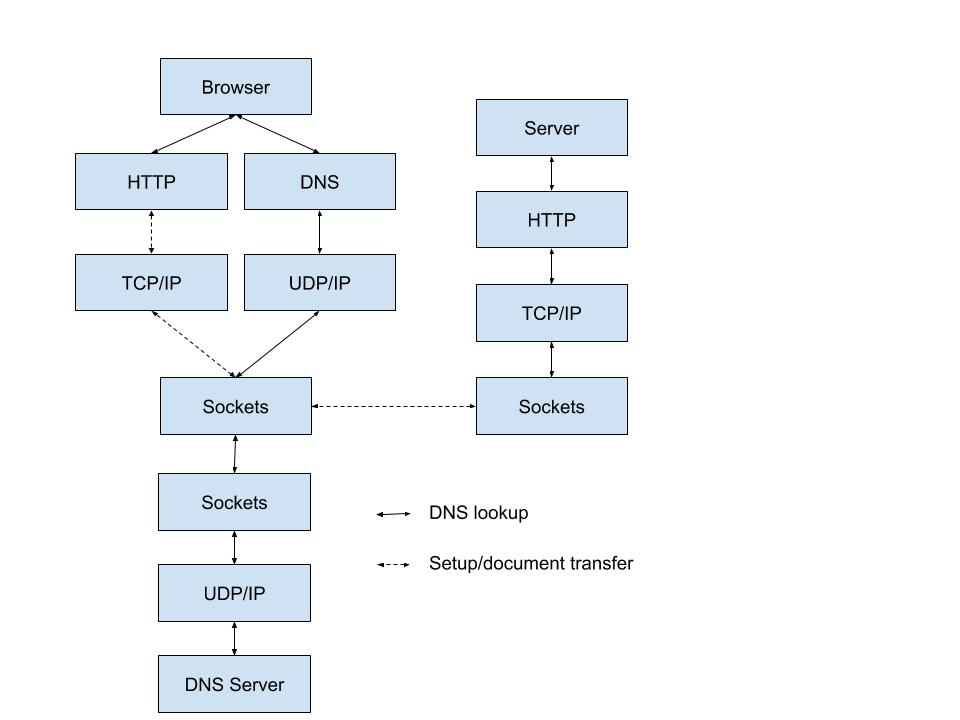
\includegraphics[scale=0.5]{HTTPlayers}
\end{sloppypar}
\begin{sloppypar}
    The requests sent to other microservices throught the network are extremely 
    slow when compared to operation within one computer as the function calls 
    would be. Therefore, the communication patterns should be changed to take 
    into account the change in communication path.
\end{sloppypar}
\begin{sloppypar}
    If the architecture is changed in such a way that the previous communication 
    model amongs the components is preserved, there would be an excessive amount 
    of communication and the resulting system is not as performant as it could 
    be \citep{fowlerlewisms}.
\end{sloppypar}


% --------------------------------------------------------------------


\section{Confidentiality}
\begin{sloppypar}
    Confidentiality in a web service is usually critical security feature. 
    There are specific services which do not nead information confidentiality 
    regarding some of the data such as public weather services and other similar data.
    Some of the information is still regarded sensitive and must be kept confidential. 
    These data can consists of personal, user, logs or other similar content.
    Users should not be able to use or view content not authorized to him/her. 
    To verify this a form of access control has to be performed. Access control 
    consists of user authentication and authorization. A user has to 
    authenticate him/her self and authorization is acquired to access to 
    information or property.
\end{sloppypar}
\begin{sloppypar}
    In an MA access control can be implemented using sessions. 
    A user authenticates using appropriate channels and a session with a session key is created. 
    The session can have an expiration time and the messages originating from 
    the user interface (UI) carry this key. Sessions and session keys can be used 
    in a distributed system which MSA is but the implementation is more difficult \citep{authinmsa}.
\end{sloppypar}

\subsection{Authentication}
\begin{sloppypar}
    In these cases where the user has to be authenticated the web service needs 
    a way to do this securily. Usually authentication is done using a tuple 
    containing user credentials i.e. a username and a password for the user. The
    user is authenticated and a key or token is transmitted to the user via the 
    network. This communication should in both MA and MSA be encrypted in a way 
    that none of the actors in the transfer path can intercept the message and 
    be able to use the credentials.
\end{sloppypar}
\begin{sloppypar}
    The credential counterparts i.e. shared secret by the server and the user 
    have to be available for the web service for verification. When using MSA 
    the service should own it's own data. When ever such information is 
    available it is a target for thieves and hackers. The services in MSA are 
    to be individually deployable and the service scalable. Authentication 
    service implementation has to take this into account. The service has to 
    adhere to practices that minimize the risks of data breaches. 
\end{sloppypar}
    
\subsubsection{Attacks}
\begin{sloppypar}
    Authentication can be attacked by a multitude of methods.     
    \begin{itemize}
        \item Cracking
        \item Impersonation attacks
        \item Hacking the system
        \item Malware
        \item Social engineering
        \item Cracking the encryption on the communication channel exchanging credentials and keys or tokens.
    \end{itemize}
\end{sloppypar}
\begin{sloppypar}
    From 2013 onwards malware and data breaches performed by hackers have 
    increased and the scale of the damage is massive. The user data containing 
    also the user passwords or hash thereof is valuable commodity which can be 
    traded in the black markets. The damage of the dataloss can be susbtantial. 
    The estimated value from the Yahoo data breach is over \$440 billion. The 
    attacks seem to have been targeted to entities with valuable data and 
    also to such targets that are lacking secure infrastructure. The least likely 
    target to be hacked where non profit organisations and the most likely were 
    medical related organizations \citep{breach}.
\end{sloppypar}
\begin{sloppypar}
    The hacked account credentials have to some extent been available for download 
    from the web. \citet{pwned} created a service where everyone can verify 
    whether any of their accounts are amogst the ones added to the service. 
    The service named as "';-- have i been pwned ?" allows users to enter their 
    username or password to the site and see a result.
\end{sloppypar}

\subsection{Authorization}
\begin{sloppypar}
    Authorization of the user rights can be implemented in various ways. One of 
    which is an authorization service which can contain the access control 
    matrix. Services being accessed verify from the authorization service that
    a particular user or the role that the user has can access the requested 
    service or functionality.
\end{sloppypar}
\begin{sloppypar}
    In a MA the access rights to a functionality can be implemented using
    annotations within the source code. This can be effective since the 
    verification can be done in memory or atleast without network communication. 
    If a session is used it can contain the information needed to verify access 
    rights.
\end{sloppypar}
\begin{sloppypar}
    In contrast to the MA in the MSA the access control matrix or matrices can't 
    be as easily accessed. In order to verify that a specific right exists the 
    service would have communicate with the authorization service every time a user
    tries to access a functionality with access restrictions. This could 
    potentially lead to an extremely lively communication from all the services 
    a formation of a bottleneck to the service.
\end{sloppypar}
\begin{sloppypar}
    https://techbeacon.com/security/microservices-apps-do-identity-access-management-without-overhead
\end{sloppypar}

\subsection{Interaction Paradigms}
\begin{sloppypar}
    As already discussed in an MA the service components can communicate using 
    events, procedure calls or other methods available within a single server 
    machine. Usually all this communication stays within a single computer and 
    thus does not necessarily compromise confidentiality.
\end{sloppypar}
\begin{sloppypar}
    In MSA single services communicate via a network.
    TODO

    Next messaging systems list is from \citep{secchalmsa}:
lightweight
-
    REST API,
    Sync RPC,
    GraphQl
    -
    Async REST,
    gRPC
    - 
    Apache Kafka,
    ZeroMQ
    -
    Java Message Service:
    1 ActiveMQ,
    2 JBOSS messaging,
    3 Glassfish
    -
    AMQP:
    1 RabbitMQ,
    2 Qpid,
    3 HornetQ
    -
    MuleESB,
    Apache ServiceMix,
    JBossESB
-
heavyweight
    WebSocket
\end{sloppypar}

\subsubsection{Representational State Transfer (REST)}
\begin{sloppypar}
    \citet{restroy} presented REST in 2000 and it has become very successfull. 
    The architectural style is was derived using various constraints one of 
    which is the demand of stateless communication. The communication i.e. 
    the request must contain all information for the server to fullfil the request. 
    All session state is stored in the client of which the server has no prior 
    knowledge before a request.
\end{sloppypar}
\begin{sloppypar}
    In her doctoral thesis \citet{secchalmsa} critiques the REST paradigm from 
    the security perspective. She states that the design of the architecture 
    does not meet the security requirements for web applications. The 
    statelessness of REST does not allow for any server side sessions and thus 
    making e.g. token repudiation impossible due to not being able to verify 
    tokens other than the correct issuer by signature and the validity. As such 
    tokens are more compatible with REST but there still has to be the private 
    keys in the server for signature verification.
\end{sloppypar}

\subsubsection{Event-Driven Communication}
\begin{sloppypar}
    
\end{sloppypar}

\subsubsection{Effects on Confidentiality}
\begin{sloppypar}
    
\end{sloppypar}

\subsubsection{Example case}
\begin{sloppypar}
    
\end{sloppypar}


% --------------------------------------------------------------------


\section{Integrity}
\begin{sloppypar}
    Information integrity in an MA web service is usually left to a single database 
    and sound architectural choices (REALLY? SOURCE).
    Transactions can be used when updating database constents to make sure that
    atomicity, consistency, isolation, and durability (ACID) \citep{acid} is followed.
    When using MSA according to the definition each of the micro services should contain 
    or have access to it's own data i.e. database. This leads to extreme difficulties in information integrity.
    TODO
\end{sloppypar}

\subsection{Introduction}
\begin{sloppypar}

\end{sloppypar}

\subsection{Effects on Integrity}
\begin{sloppypar}

\end{sloppypar}

\subsection{Example case}
\begin{sloppypar}

\end{sloppypar}

\subsection{Threats}
\begin{sloppypar}

\end{sloppypar}


% --------------------------------------------------------------------


\section{Availability}
\begin{sloppypar}
    Availability in this web service context is defined as such that the property or information 
    is available when it is needed.
\end{sloppypar}

\subsection{Possible Attacks}
\begin{sloppypar}
    D-o-S 
\end{sloppypar}

\subsection{Comparison}
\begin{sloppypar}
    
\end{sloppypar}

\subsection{Introduction}
\begin{sloppypar}

\end{sloppypar}

\subsection{Effects on Availability}
\begin{sloppypar}

\end{sloppypar}

\subsection{Example case}
\begin{sloppypar}

\end{sloppypar}


% --------------------------------------------------------------------


\section{Other MSA specific security matters}
\begin{sloppypar}

\end{sloppypar}

\subsection{Platforms}
\begin{sloppypar}
    Docker Swarm
    Kubernetes (K8s)
    Azure
    
    sandbox
    virtualization 
\end{sloppypar}

\subsection{Monitoring and logging}
\begin{sloppypar}

\end{sloppypar}

\subsection{Software Development}
\begin{sloppypar}

\end{sloppypar}

\subsection{Deployment and Operation}
\begin{sloppypar}
    Developing software using the MA the structure the whole application or service 
    is usually deployed as a whole and the program code can be compiled, tested 
    and used as a single unit or multiple modules. In contrast to this a service 
    implemented by using a MSA can be deployed in single microservice units and 
    thus a single service can be worked upon individually and deployed once ready.
\end{sloppypar}
\begin{sloppypar}
    The immediacy in the deployment of the microservices entail a very specific 
    security risk. In a paper \citet{integinside} present threats from malicious 
    insiders working on the services as developers or other positions with access
    to sensitive information. In microservice development the finished 
    implementations are to be immediately released to production. There are few 
    steps in the CD pipeline prior to this but once tests pass in the test 
    environments the pipeline is supposed to publish the changes to the actual 
    production environment. The paper presents four specific threats. The first 
    one is that the knowledge of sensitive information is spread among the 
    developers more widely than in MA. The developers need access to be able to 
    produce working solutions. The second threat is that the insiders 
    monitoring and operating the running system intentionally harm the system 
    by making malicious changes. The third threat is the developers knowing the 
    configurations and their ability to make almost instat changes to them or 
    the microservices them selves. The last presented threat in the paper is the 
    non-repudiation. The system is not able to dis-allow malicious requests 
    when the developers have had access to the keys and other configurations. 
    They can effectively implement services or requests that emit malicious 
    requests or responds.
\end{sloppypar}
\begin{sloppypar}
    Malicious attempts in a MA are more easily screened by performing security
    audits and by peer reviewing the code. In a MSA the knowledge of a single 
    service and it's inner workings are shared by a more limited number of people.
    Finding the compromised actions from the interoperability of the distinct 
    microservices is a daunting task.
\end{sloppypar}
\begin{sloppypar}
    
\end{sloppypar}

\subsection{Service discovery}
\begin{sloppypar}
    The MSA can have a service discovery service into which all available services 
    can register them selves.
    https://www.nginx.com/blog/service-discovery-in-a-microservices-architecture/
    https://www.consul.io
\end{sloppypar}

\subsection{Externalized configuration}
\begin{sloppypar}
    To allow for easy configuration change management there should exist a 
    configuration orchestration service. This service should have an API from 
    which services in their startup can load their appropriate configuration. 
    The configuration of the whole system can be easily maintained through the 
    API.
\end{sloppypar}
\begin{sloppypar}
    The contents of the configuration is highly sensitive information. It 
    consists of addressess, credentials and other information that alter 
    the behaviour of the system. Therefore, the content must be stored safely 
    and not allowed to be read or altered by unauthorized users.
\end{sloppypar}




% --------------------------------------------------------------------
% --------------------------------------------------------------------

\section{Conclusion}
\begin{sloppypar}

\end{sloppypar}


% Loppuluku päättää työn. Luvun nimi on tyypillisesti ``yhteenveto'' tai
% ``johtopäätöksiä''. Valitse se otsikko, joka tuntuu sopivammalta työsi
% luonteeseen. Joka tapauksessa loppuluku sisältää niin työn yhteenvedon
% kuin johtopäätöksiä työn tulosten perusteella. Pääajatus on antaa
% lukijalle selvä kuva siitä, miten johdannossa asetettuihin
% tavoitteisiin työssä vastattiin.

% Käsittele loppupuvussa seuraavia asioita (jotakuinkin tässä järjestyksessä):
% %
% \begin{itemize}
%   \item Muistutus työn tavoitteista (sidoksisuus johdantoon)
%   \item Päätulokset kootaan yhteen, pohditaan niiden merkitystä
%   \item Suositukset konkreettisiksi toimenpiteiksi (``Mitä sitten?'' 
% Nyt kun käytössä on tämän työn myötä tullut tieto, 
% mitä se nyt tarkoittaa tälle asialle/alalle.)
%   \item Tulosten soveltuvuus, käyttöön liittyvät rajoitukset
%   \item Jatkotutkimustarve 
% (``Tulevaisuudessa olisi mielenkiintoista selvittää...'' tms.)
%   \item Työn onnistumisen arviointi 
% (Huom! Älä arvioi omaa kirjoitusprosessiasi vaan tekemääsi tutkimusta)
% \end{itemize}

% --------------------------------------------------------------------


%\clearpage                     % luku loppuu, loput kelluvat tänne, sivunv.

%\input{luku2}                  % tässä tyylissä ei sivunvaihtoja lukujen
%\input{luku3}                  %   välillä. Toiset ohjaajat haluavat 
%\input{luku4}                  %   sivunvaihdot.

\label{pages:text}
\clearpage                     % luku loppuu, loput kelluvat tänne, sivunvaihto
%\newpage                       % ellei ylempi tehoa, pakota lähdeluettelo 
                               % alkamaan uudelta sivulta

% -------------- Lähdeluettelo / reference list -----------------------
%
% Lähdeluettelo alkaa aina omalta sivultaan; pakota lähteet alkamaan
% joko \clearpage tai \newpage
%
%
% Muista, että saat kirjallisuusluettelon vasta
%  kun olet kääntänyt ja kaulinnut "latex, bibtex, latex, latex"
%  (ellet käytä Makefilea ja "make")

% Viitetyylitiedosto aaltosci_t.bst; muokattu HY:n tktl-tyylistä.
\bibliographystyle{aaltosci_t}
% Katso myös tämän tiedoston yläosan "preamble" ja siellä \bibpunct.

% Muutetaan otsikko "Kirjallisuutta" -> "Lähteet"
\renewcommand{\refname}{\REFERENCES}  % article-tyyppisen
%\renewcommand{\bibname}{Lähteet}  % jos olisi book, report-tyyppinen

% Lisätään sisällysluetteloon
\addcontentsline{toc}{section}{\refname}  % article
%\addcontentsline{toc}{chapter}{\bibname}  % book, report

% Määritä kaikki bib-tiedostot
\bibliography{lahteet}
%\bibliography{thesis_sources,ietf_sources}

\label{pages:refs}
\clearpage         % erotetaan mahd. liitteet alkamaan uudelta sivulta

% -------------- Liitteet / Appendices --------------------------------
%
% Liitteitä ei yleensä tarvita. Kommentoi tällöin seuraavat
% rivit.

% Tiivistelmässä joskus matemaattisen kaavan tarkempi johtaminen, 
% haastattelurunko, kyselypohja, ylimääräisiä kuvia, lyhyitä 
% ohjelmakoodeja tai datatiedostoja.

\appendix
%\section{Esimerkkiliite}
\label{sec:app1}

Jos työhön kuuluu suurikokoisia (yli puoli sivua) kuvia, taulukoita
tai karttoja tms., jotka eivät kokonsa puolesta sovi tekstin joukkoon,
ne laitetaan liitteisiin. Liitteet numeroidaan. Jokaiseen liitteeseen
tulee viitata tekstissä, eikä liitteisiin ole tarkoitus laittaa ``mitä
tahansa'', vaan vain työlle oikeasti tarpeellista
materiaalia. Liitteisiin voidaan sijoittaa esim. malli
kyselylomakkeesta, jolla tutkimushaastattelu toteutettiin,
pohjapiirustuksia, taulukoita, kaavioita, kuvia tms.

\textbf{TIK.kand suositus: Vältä liitteitä.} Jos iso kuva, mieti onko
sen koko pienettävissä (täytyy olla tulkittavissa) normaalin tekstin
yhteyteen. Joskus liitteeksi lisätään matemaattisen kaavan tarkempi
johtaminen, haastattelurunko, kyselypohja, ylimääräisiä kuvia, lyhyitä
ohjelmakoodeja tai datatiedostoja.

Työtä varten mahdollisesti tehtyjä ohjelmakoodeja ei tyypillisesti
lisätä tänne, ellei siihen ole joku erityinen syy. (Kukaan ei ala
kirjoittaa tai tarkistamaan koko koodia paperilta vaan pyytää sitä
sinulta, jos on kiinnostunut.)

%\subsection{Esimerkkiliitteen otsikko 1}
%\label{sec:app1_1}
%
%Kerätty data-aineisto.
%
% -------------------------------------------------------------- %
%
%\newpage
%\section{Toinen esimerkkiliite}
%\label{sec:app2}
%
%Haastattelukysymykset: mitä, missä, milloin, kuka, miten.



\label{pages:appendices}

% ---------------------------------------------------------------------

\end{document}
